\chapter{Projectactiviteiten}
\section{Mijlpalen}
Hieronder bevindt zich de planning voor het gehele project. De genoemde data zijn de deadlines voor oplevering en reflecteren niet de werkelijke inleverdatum.

\begin{tabular}{ r | c r }
  Teamcontract & 11-11-2015 (Week 1) \\
  Github Repo (met bijbehorende mappen) & 11-11-2015 (Week 1) \\
  Interview Opdrachtgever & 30-11-2015 (Week 3) \\
  Plan van Aanpak & 02-12-2015 (Week 4) \\
  Requirements Document (MoSCoW) & 01-12-2015 (Week 4) \\
  Requirements Architechture &  09-12-2015 (Week 5) \\
  Solution Architechture & 16-12-2015 (Week 6) \\
  Technisch Verslag	& (Week 7 / Projectweek 1) \\
  Eindproduct (software + hardware)	& 22-01-2016 \\
\end{tabular}

\section{Planning}
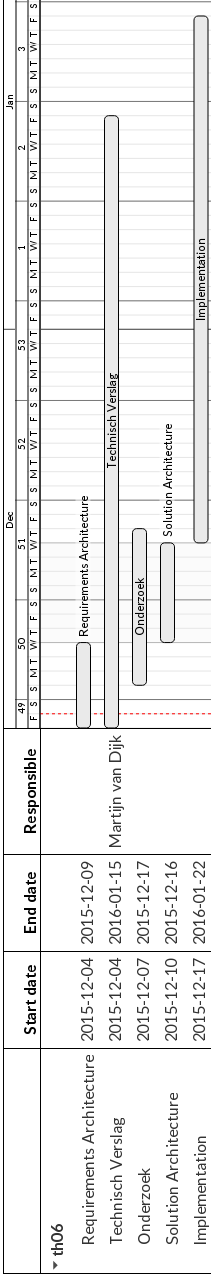
\includegraphics[width=3.55cm]{planning.png}
\newpage
De bovenstaande planning is een screenshot van de OpenProject Web interface. De interactieve versie is te vinden op \url{https://project-th06.martijnvandijk.net/projects/th06/timelines/2}. Dit is een afgeschermde omgeving. Op verzoek kunnen er voor docenten login credentials aangemaakt worden.

\section{Verantwoordelijkheden}
\begin{tabular}{ p{5cm} | l }
\textbf{Deelproduct of taak} & \textbf{Eindverantwoordelijke}\\
\hline
\multicolumn{2}{c}{Documentatie}\\
\hline
Onderzoek & Christiaan van den Berg \\
Plan van Aanpak & Martijn van Dijk \\
Requirements Document & Chiel Douwes \\
Requirements Architecture & Christiaan van den Berg \\
Solution Architecture & Aydin Biber \\
Technisch Verslag & Martijn van Dijk \\
\hline
\multicolumn{2}{c}{Software}\\
\hline
Webinterface & Aydin Biber\\
Low-level interfacing met hardware & Martijn van Dijk\\
Demonstratie \& Presentatie & Chiel Douwes \\
\end{tabular}